\chapter{Specifikace cílů práce}

Účelem této sekce je stanovení přesného popisu řešené problematiky a cílů práce. Tyto cíle popíšeme formou požadavků na výsledky práce. Při specifikaci požadavků budeme vycházet ze zadání. Na základě zadání můžeme specifikovat tři oblasti požadavků.

V první oblasti se budeme zabývat požadavky na rešeršní části práce -- analýzu \emph{principů} používaných při \emph{objektově orientovaném návrhu a implementaci}. Část druhá bude obsahovat požadavky na \emph{formalizaci pravidel}, která umožní popsat principy analyzované v části první. Třetí část poskytne rozbor \emph{požadavků na systém}, který by měl demonstrovat vyhodnocování/validaci definovaných pravidel na existujících zdrojových kódech.

Na konci kapitoly rozebereme v rámci jedné sekce existující podobná řešení/nástroje, jejich výhody a nevýhody.

\section{Požadavky na analýzu základních návrhových principů}

TODO: zpracovat
popsat, které návrhové principy budeme analyzovat a z jakého úhlu pohledu

\begin{itemize}
\item rozbor základních principů používaných při objektově orientovaném návrhu a implementaci, konkrétně low coupling, high cohesion a Law of Demeter
\end{itemize}

\section{Požadavky na formalizaci pravidel}

\begin{itemize}
\item vhodně definovat problémovou doménu -- objekty nad nimiž budeme pracovat a základní vztahy mezi nimi
\item definovat jazyk pro zadávání pravidel a specifikace pravidel pro návrhové principy \emph{Law of Demeter}, \emph{low coupling} a \emph{high cohesion}
\end{itemize}

\section{Požadavky na systém pro vyhodnocování pravidel}

TODO: rephrase

Vytvoření nástroje, který umožní, který umožní ověřovat pravidla v existujícím zdrojovém kódu
Globální struktura výsledné práce je na obrázku \ref{requirements-system_structure}.

\begin{figure}[h!]
  \centering
  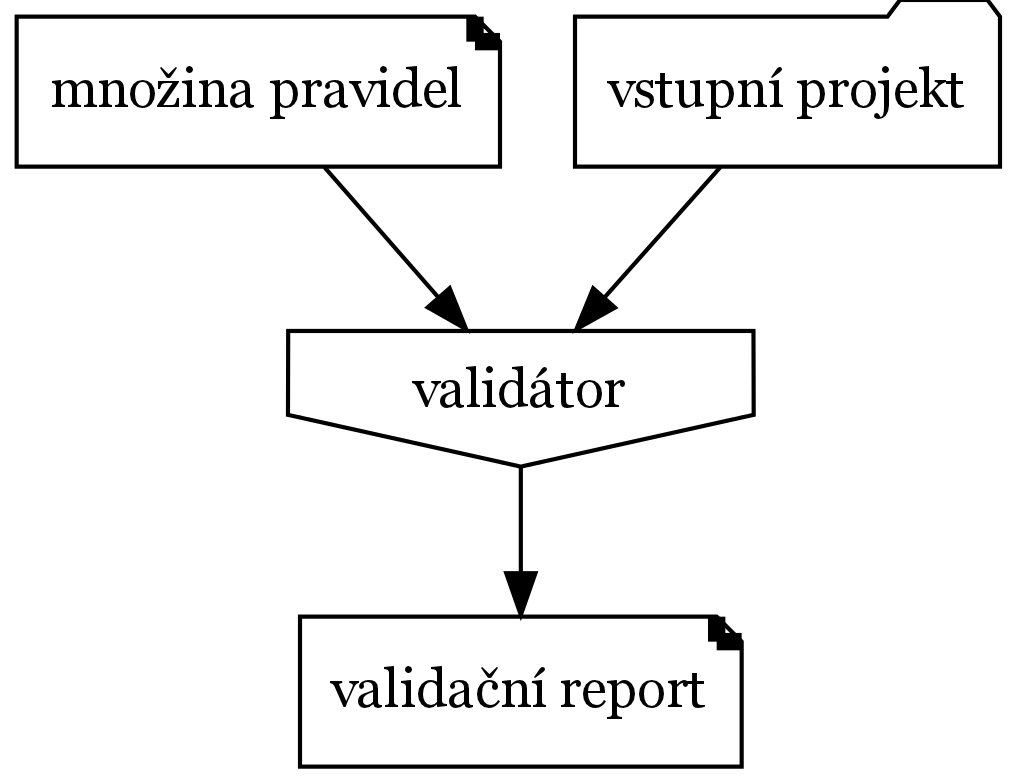
\includegraphics[width=0.5\textwidth]{./graphs/global_structure.png}
  \caption{Struktura systému.\label{requirements-system_structure}}
\end{figure}

\subsection{Funkční požadavky na výsledný systém}
\begin{itemize}
\item průběžná kontrola projektu a výpis zjištěných porušení pravidel (validace) do výstupního souboru
\item provedení kontroly \uv{on demand} -- uživatel stiskne tlačítko, provede se kontrola projektu proti pravidlům a výstup se zobrazí ve výstupním souboru (např. konzoli)
\end{itemize}

\subsection{Nefunkční požadavky na výsledný systém}
\begin{itemize}
\item systém bude fungovat nad instancemi programovacího jazyka Java 6 (projekty napsané v jazyku Java)
\item systém bude umožňovat definovat další pravidla (požadavek rozšiřitelnosti ze zadání)
\end{itemize}

\section{Rešerše existujících řešení}
\label{requirements-existing_tools}

TODO: možná přidat i rešerši exisujících formalizací pro návrh software (Z-notation, UPPAAL, etc.)

TODO: provest resersi o tom, co vsechny tyto nastroje umi, jejich pozitiva a negativa

TODO: v rychlosti zopakovat rešerši na nové nástroje a konkrétní vlastnosti, které jsou důležité pro tuto práci

\subsection{JDepend}

\begin{itemize}
\item \href{http://www.clarkware.com/software/JDepend.html}{http://www.clarkware.com/software/JDepend.html}
\item nástroj pro testování kvality návrhu
\item pracuje nad \verb+*.class+ soubory (získává data z bytekódu)
\end{itemize}

\subsection{QJ-Pro}
\begin{itemize}
\item \href{http://qjpro.sourceforge.net}{http://qjpro.sourceforge.net}
\end{itemize}

\subsection{DP-Miner}
\begin{itemize}
\item \href{http://www.utdallas.edu/~yxz045100/DesignPattern/DP\_Miner/}{http://www.utdallas.edu/~yxz045100/DesignPattern/DP\_Miner/}
\item hledání návrhových vzorů v existujících projektech
\item článek: Jing Dong and Yajing Zhao, Experiments on Design Pattern Discovery \\ (\href{http://www.utdallas.edu/~jdong/papers/PROMISE07.pdf}{http://www.utdallas.edu/~jdong/papers/PROMISE07.pdf})
\end{itemize}

\subsection{Macker}
\begin{itemize}
\item \href{http://innig.net/macker/}{http://innig.net/macker/}
\item build-time architectural rule checking utility for Java developers
\item zpracovává \verb+*.class+ soubory (bytekód)
\end{itemize}

TODO: complete research on following tools:

\subsection{Squale}
\begin{itemize}
\item \href{http://www.squale.org/}{http://www.squale.org/}
\end{itemize}

\subsection{FindBugs}
\begin{itemize}
\item \href{http://findbugs.sourceforge.net/}{http://findbugs.sourceforge.net/}
\end{itemize}

\subsection{CheckStyle}
\begin{itemize}
\item \href{http://checkstyle.sourceforge.net/}{http://checkstyle.sourceforge.net/}
\end{itemize}

\subsection{PMD}
\begin{itemize}
\item \href{http://pmd.sourceforge.net/}{http://pmd.sourceforge.net/}
\end{itemize}

\subsection{Soot}
\begin{itemize}
\item \href{http://www.sable.mcgill.ca/soot/}{http://www.sable.mcgill.ca/soot/}
\item Soot: a Java Optimization Framework
\end{itemize}
